\documentclass[a4paper,12pt]{article}
\usepackage[english,ukrainian,russian]{babel}
\linespread{1}
\usepackage{ucs}
\usepackage[utf8]{inputenc}
\usepackage[T2A]{fontenc}
\usepackage[paper=portrait,pagesize]{typearea}
\usepackage{amsmath}
\usepackage{bigints}
\usepackage{amsfonts}
\usepackage{graphicx}
\usepackage{amssymb}
\usepackage{cancel}
\usepackage{gensymb}
\usepackage{multirow}
\usepackage{rotate} 
\usepackage{pdflscape}
\usepackage{bigstrut}
\usepackage[pageanchor]{hyperref}
\usepackage{chngpage}
\newcommand{\dx}{\textbf{d}x}
\newcommand{\dt}{\textbf{d}t}
\newcommand{\du}{\textbf{d}u}
\newcommand{\dv}{\textbf{d}v}
\newcommand{\dy}{\textbf{d}y}
\newcommand{\ds}{\textbf{d}s}
\newcommand{\dz}{\textbf{d}z}
\newcommand{\arch}{\textrm{arcch}}
\newcommand{\arsh}{\textrm{arcsh}}
\newcommand{\dint}{\displaystyle\int}
\newcommand\tab[1][1cm]{\hspace*{#1}}
\newcommand{\dsum}{\displaystyle\sum}
\usepackage[left=20mm, top=20mm, right=15mm, bottom=15mm, nohead, nofoot]{geometry}
\usepackage{verbatim}

\usepackage{listings}
\usepackage{xcolor}

\definecolor{codegreen}{rgb}{0,0.6,0}
\definecolor{codegray}{rgb}{0.5,0.5,0.5}
\definecolor{codepurple}{rgb}{0.58,0,0.82}
\definecolor{backcolour}{rgb}{0.95,0.95,0.92}

\lstdefinestyle{mystyle}{
	backgroundcolor=\color{backcolour},   
	commentstyle=\color{codegreen},
	keywordstyle=\color{blue},
	numberstyle=\tiny\color{codegray},
	stringstyle=\color{red},
	basicstyle=\ttfamily\footnotesize,
	breakatwhitespace=false,         
	breaklines=true,                 
	captionpos=b,                    
	keepspaces=true,                 
	numbers=none,                    
	numbersep=5pt,                  
	showspaces=false,                
	showstringspaces=false,
	showtabs=false,                  
	tabsize=4,
	frame=shadowbox
}

\lstset{style=mystyle}

\begin{document}
	
		\begin{center}
		%\vspace*{0,1cm}
		{\Large \bfseries \textsc{Лабораторна робота №2}}\\
		\hrulefill\\
		\Large \textsc{ФІ-12 Завалій Олександр\\ Варіант №5}
	\end{center}
	\begin{center}
		\section*{\bfseries{Завдання}}
	\end{center} 
	\textbf{Предметна область:} \\
	Навчально-методичне управління (облік площі приміщень). \\
	\textbf{Основні предметно-значущі сутності:} \\
	Приміщення, Підрозділи. \\
	\textbf{Основні предметно-значущі атрибути сутностей:}
	\begin{enumerate}
		\item[-] \textbf{Приміщення}: назва або номер приміщення, вид приміщення (аудиторія, кабінет і т.п.), площа, кількість посадочних місць, підрозділ. 
		\item[-] \textbf{Підрозділи}: назва, вид підрозділу.
	\end{enumerate}
	\textbf{Основні вимоги до функцій системи:}
	\begin{enumerate}
		\item[-] Вибрати назви або номери приміщень за підрозділами;
		\item[-] Підрахувати загальну площу навчальних аудиторій по приміщеннях і в цілому по навчальному закладу;
		\item[-] Підрахувати загальну кількість посадочних місць для співробітників по підрозділам.
	\end{enumerate}
	\textbf{Тригери:}
	\begin{enumerate}
		\item На видалення запису з таблиці «Приміщення». Якщо для приміщення зазначено підрозділ, заборонити видалення запису.
		\item Створити представлення «Аудиторії» з полями «код приміщення», «назва приміщення», «підрозділ», в яку повинні входити приміщення виду «Аудиторія». Оновлювати представлення «Аудиторії».
	\end{enumerate}
	\textbf{Процедура:}\\
	Процедура повинна повертати кількість приміщень для зазначеного підрозділу. \\
	\begin{center}
		\textbf{Завдання для лабораторної роботи}
	\end{center}
	\begin{enumerate}
		\item Введіть обмеження на границі допустимих значень створеної вами бази даних.
		\item Створіть зовнішні ключі у всіх таблицях, використовуючи опцію FOREIGN KEY, при цьому встановіть опцію каскадного видалення там, де це необхідно.
		\item Відключіть обмеження зовнішнього ключа в таблиці . введіть в таблицю запис, значення поля якого порушує логічну цілісність таблиці. Спробуйте підключити раніше відключені обмеження.
		\item Виконайте всі необхідні дії для того, щоб знову підключити обмеження, а всі дані у відношенні відповідали умовам цілісності бази даних.
\newpage
		\item Змоделюйте ситуацію, коли необхідно відключити обмеження та розробіть заходи, які дозволять вам в подальшому привести базу даних в стан, що відповідає всім умовам цілісності.
		\item Додати в одну з таблиць стовпець Single, тип даних VARCHAR(3), призначивши значення по замовчуванню «так». Видалити стовпець.
		\item Перейменувати одну з таблиць.
		\item Повернути попередню назву перейменованої таблиці. 
	\end{enumerate}
	
	
	\begin{center}
		\section*{\bfseries{Реалізація завдання}}
	\end{center}
	
	%\lstinputlisting[language=SQL]{Code.txt}
	\begin{lstlisting}[language=SQL]
	USE master
	CREATE DATABASE TestProject
	GO
	USE TestProject
	
	CREATE TABLE Ownerss(
		OwnerId INT IDENTITY PRIMARY KEY,
		FirstName VARCHAR(50) NOT NULL,
		LastName VARCHAR(50) NOT NULL );
	
	CREATE TABLE Building(
		BiuldingId INT IDENTITY PRIMARY KEY,
		OwnerId INT NOT NULL,
		TypeOfBuilding VARCHAR(50) NOT NULL,
		AmountOfRooms INT CHECK (AmountOfRooms BETWEEN 2 AND 40),
		AmountOfFloors INT NOT NULL); 
	
	CREATE TABLE Subdivision(
		SubdivisionId INT IDENTITY PRIMARY KEY,
		SubdivisionName VARCHAR(50) UNIQUE NOT NULL,
		SubdivisionType VARCHAR(50) NOT NULL );
	
	CREATE TABLE TypeOfSeats(
		SeatsId INT IDENTITY PRIMARY KEY,
		TypeOfSeats VARCHAR(50) UNIQUE NOT NULL,
		SeatMaterial VARCHAR(50) NOT NULL ); 
	
	CREATE TABLE Room(
		RoomId INT IDENTITY PRIMARY KEY,
		TypeOfRoom VARCHAR(50) NOT NULL,
		Area INT NOT NULL, 
		AmountOfSeats INT NOT NULL, 
		Storey INT NOT NULL,
		RoomNumber INT UNIQUE NOT NULL,
		SeatsId int, 
		SubdivisionId INT NOT NULL,
		BiuldingId INT NOT NULL );
	
	CREATE TABLE RoomSeats(
		RoomId INT FOREIGN KEY REFERENCES Room(RoomId),
		SeatsId INT FOREIGN KEY REFERENCES TypeOfSeats(SeatsId),
		PRIMARY KEY(RoomId, SeatsId) );
	\end{lstlisting}
\newpage
	\begin{center}
		\textbf{№1}
	\end{center}
	\begin{lstlisting}[language=SQL]
	ALTER TABLE Room
		ADD CONSTRAINT Size_of_area CHECK (Area BETWEEN 10 AND 350);
	ALTER TABLE Room
		ADD CONSTRAINT Amount_of_seats CHECK (AmountOfSeats BETWEEN 0 AND 200);
	ALTER TABLE Room
		ADD CONSTRAINT Amount_of_storey CHECK (Storey BETWEEN 1 AND 10);
	ALTER TABLE Building
		ADD CONSTRAINT Amount_of_floors CHECK (AmountOfFloors BETWEEN 1 AND 10);
	\end{lstlisting}
	\begin{center}
		\textbf{№2}
	\end{center}
	\begin{lstlisting}[language=SQL]
	ALTER TABLE Room
		ADD CONSTRAINT Error_subdivision_id FOREIGN KEY (SubdivisionId) 
		REFERENCES Subdivision (SubdivisionId) ON DELETE CASCADE ,
		CONSTRAINT Error_biulding_id FOREIGN KEY (BiuldingId) 
		REFERENCES Building (BiuldingId) ON DELETE CASCADE;
	
	ALTER TABLE Building
		ADD CONSTRAINT Error_owner_id FOREIGN KEY (OwnerId) 
		REFERENCES Ownerss (OwnerId);
	\end{lstlisting}
	\begin{center}
		\textbf{№3}
	\end{center}
	\begin{lstlisting}[language=SQL]
	ALTER TABLE Room
		NOCHECK CONSTRAINT Size_of_area
	
	INSERT INTO Ownerss (FirstName, LastName) VALUES ('Alexandr', 'Zavalii');
	INSERT INTO Building (OwnerId, TypeOfBuilding, AmountOfRooms, AmountOfFloors) VALUES (1, 'Enterprise', 30, 3);
	INSERT INTO Subdivision (SubdivisionName, SubdivisionType) VALUES ('Lab', 'Chemical');
	INSERT INTO TypeOfSeats (TypeOfSeats, SeatMaterial) VALUES ('Armchairs','Leather');
	INSERT INTO Room (TypeOfRoom, Area, AmountOfSeats, Storey, RoomNumber, SeatsId, SubdivisionId, BiuldingId) VALUES ('The audience', 9999, 40, 1, 23, 1, 1, 1);
	INSERT INTO RoomSeats (RoomId, SeatsId) VALUES (1, 1);
	
	SELECT * FROM Room
	\end{lstlisting}
	\begin{figure}[h!]
		\centering
		\begin{minipage}[h]{1\linewidth}
			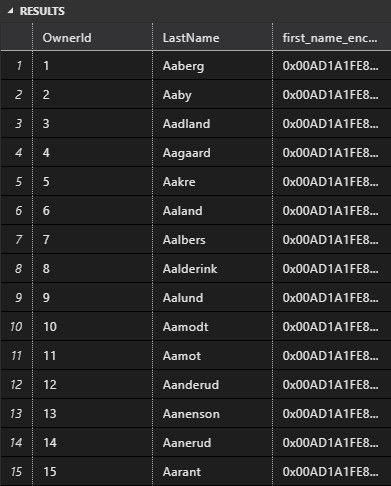
\includegraphics[width=1\linewidth]{Figure_1.jpg}  
		\end{minipage}
		\caption{Вивід таблиці з відключеним обмеженням зовнішнього ключа.}
	\end{figure}
\newpage
	\begin{lstlisting}[language=SQL]
	ALTER TABLE Room WITH CHECK
		CHECK CONSTRAINT Size_of_area
	\end{lstlisting}
	\begin{figure}[h!]
		\centering
		\begin{minipage}[h]{1.05\linewidth}
			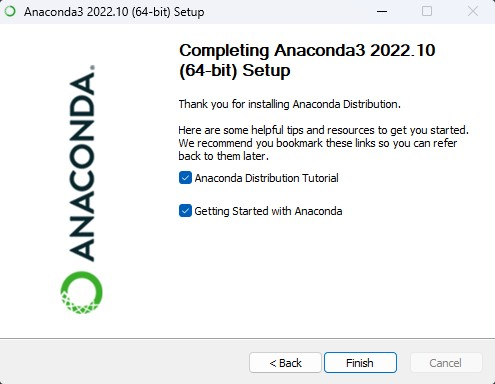
\includegraphics[width=1\linewidth]{Figure_2.jpg}  
		\end{minipage}
		\caption{Маємо помилку при спробі підключити раніше відключені обмеження.}
	\end{figure}
	\begin{center}
		\textbf{№4}
	\end{center}
	\begin{lstlisting}[language=SQL]
	UPDATE Room SET Area='350' WHERE RoomId IN (1)
	ALTER TABLE Room WITH CHECK
		CHECK CONSTRAINT Size_of_area
		
	SELECT * FROM Room
	\end{lstlisting}
	\begin{figure}[h!]
		\centering
		\begin{minipage}[h]{1.05\linewidth}
			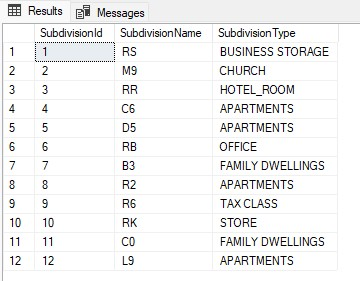
\includegraphics[width=1\linewidth]{Figure_3.jpg}  
		\end{minipage}
		\caption{Обмеження знову підключені, а всі дані у відношенні відповідають умовам цілісності бази даних.}
	\end{figure}
	\begin{center}
		\textbf{№5}
	\end{center}
	Оскільки максимальна кількість поверхів вставновлена 10, а у місті, наприклад, будують шістнадцяти повеховий будинок. Потрібно відключити старі обмеження та ввести нові.
	\begin{lstlisting}[language=SQL]
	ALTER TABLE Room DROP CONSTRAINT Amount_of_storey
	
	ALTER TABLE Building DROP CONSTRAINT Amount_of_floors
	
	ALTER TABLE Room
		ADD CONSTRAINT Amount_of_storey CHECK (Storey BETWEEN 1 AND 16)
	ALTER TABLE Building
		ADD CONSTRAINT Amount_of_floors CHECK (AmountOfFloors BETWEEN 1 AND 16)
	
	INSERT INTO Building (OwnerId, TypeOfBuilding, AmountOfRooms, AmountOfFloors) VALUES (1, 'Enterprise', 35, 15);
	INSERT INTO Room (TypeOfRoom, Area, AmountOfSeats, Storey, RoomNumber, SeatsId, SubdivisionId, BiuldingId) VALUES ('Pantry', 290, 70, 16, 29, 1, 1, 2);
	SELECT * FROM Building
	SELECT * FROM Room
	\end{lstlisting}
\newpage
	\begin{figure}[h!]
		\centering
		\begin{minipage}[h]{1.05\linewidth}
			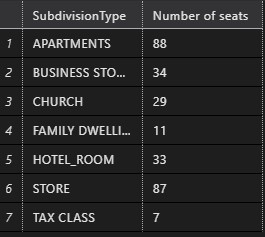
\includegraphics[width=1\linewidth]{Figure_4.jpg}  
		\end{minipage}
		\caption{Нові обмеження працюють коректно.}
	\end{figure}
	
	\begin{center}
		\textbf{№6}
	\end{center}
	\begin{lstlisting}[language=SQL]
	ALTER TABLE Subdivision
		ADD Single VARCHAR(3) NOT NULL 
		CONSTRAINT DF_Single DEFAULT 'Yes'
		WITH VALUES
	
	SELECT * FROM Subdivision
	
	ALTER TABLE Subdivision DROP CONSTRAINT DF_Single;
	ALTER TABLE Subdivision DROP COLUMN Single;
	
	SELECT * FROM Subdivision
	\end{lstlisting}
	\begin{figure}[h!]
		\centering
		\begin{minipage}[h]{0.9\linewidth}
			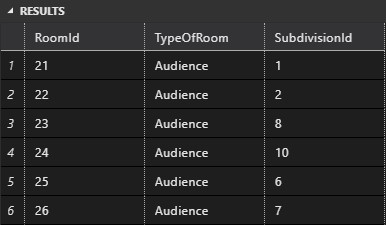
\includegraphics[width=1\linewidth]{Figure_5.jpg}  
		\end{minipage}
		\caption{Стовпець Single, тип даних VARCHAR(3), зі значенням по замовчуванню «Yes».}
		\begin{minipage}[h]{0.9\linewidth}
			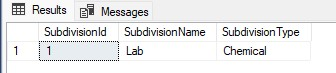
\includegraphics[width=1\linewidth]{Figure_6.jpg}  
		\end{minipage}
		\caption{Видалений стовпець Single.}
	\end{figure}
	
\newpage
	\begin{center}
		\textbf{№7}
	\end{center}
	\begin{lstlisting}[language=SQL]
	EXEC sp_rename 'dbo.Subdivision', 'Subdivision05';
	SELECT * FROM sys.objects WHERE type in (N'U')
	\end{lstlisting}
	\begin{figure}[h!]
		\centering
		\begin{minipage}[h]{0.8\linewidth}
			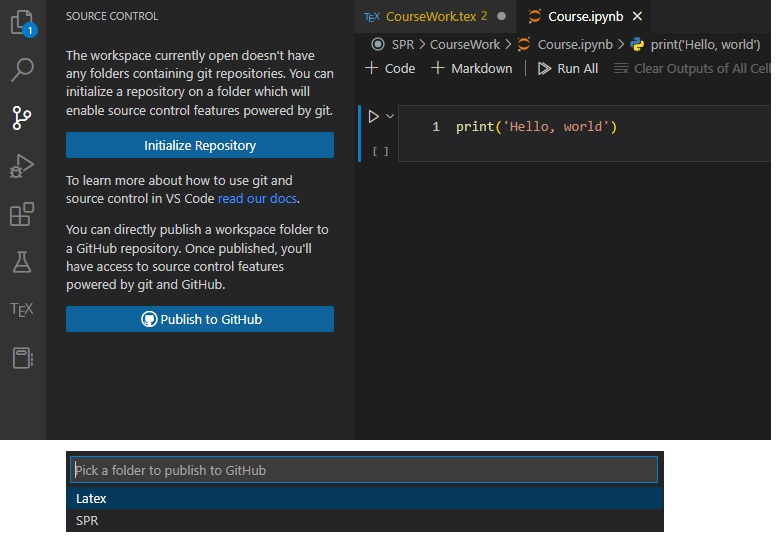
\includegraphics[width=1\linewidth]{Figure_7.jpg}  
		\end{minipage}
		\caption{Таблиця Subdivision перейменована на Subdivision05.}
	\end{figure}
	\begin{center}
		\textbf{№8}
	\end{center}
	\begin{lstlisting}[language=SQL]
	EXEC sp_rename 'dbo.Subdivision05', 'Subdivision';
	SELECT * FROM sys.objects WHERE type in (N'U')
	\end{lstlisting}
	\begin{figure}[h!]
		\centering
		\begin{minipage}[h]{0.8\linewidth}
			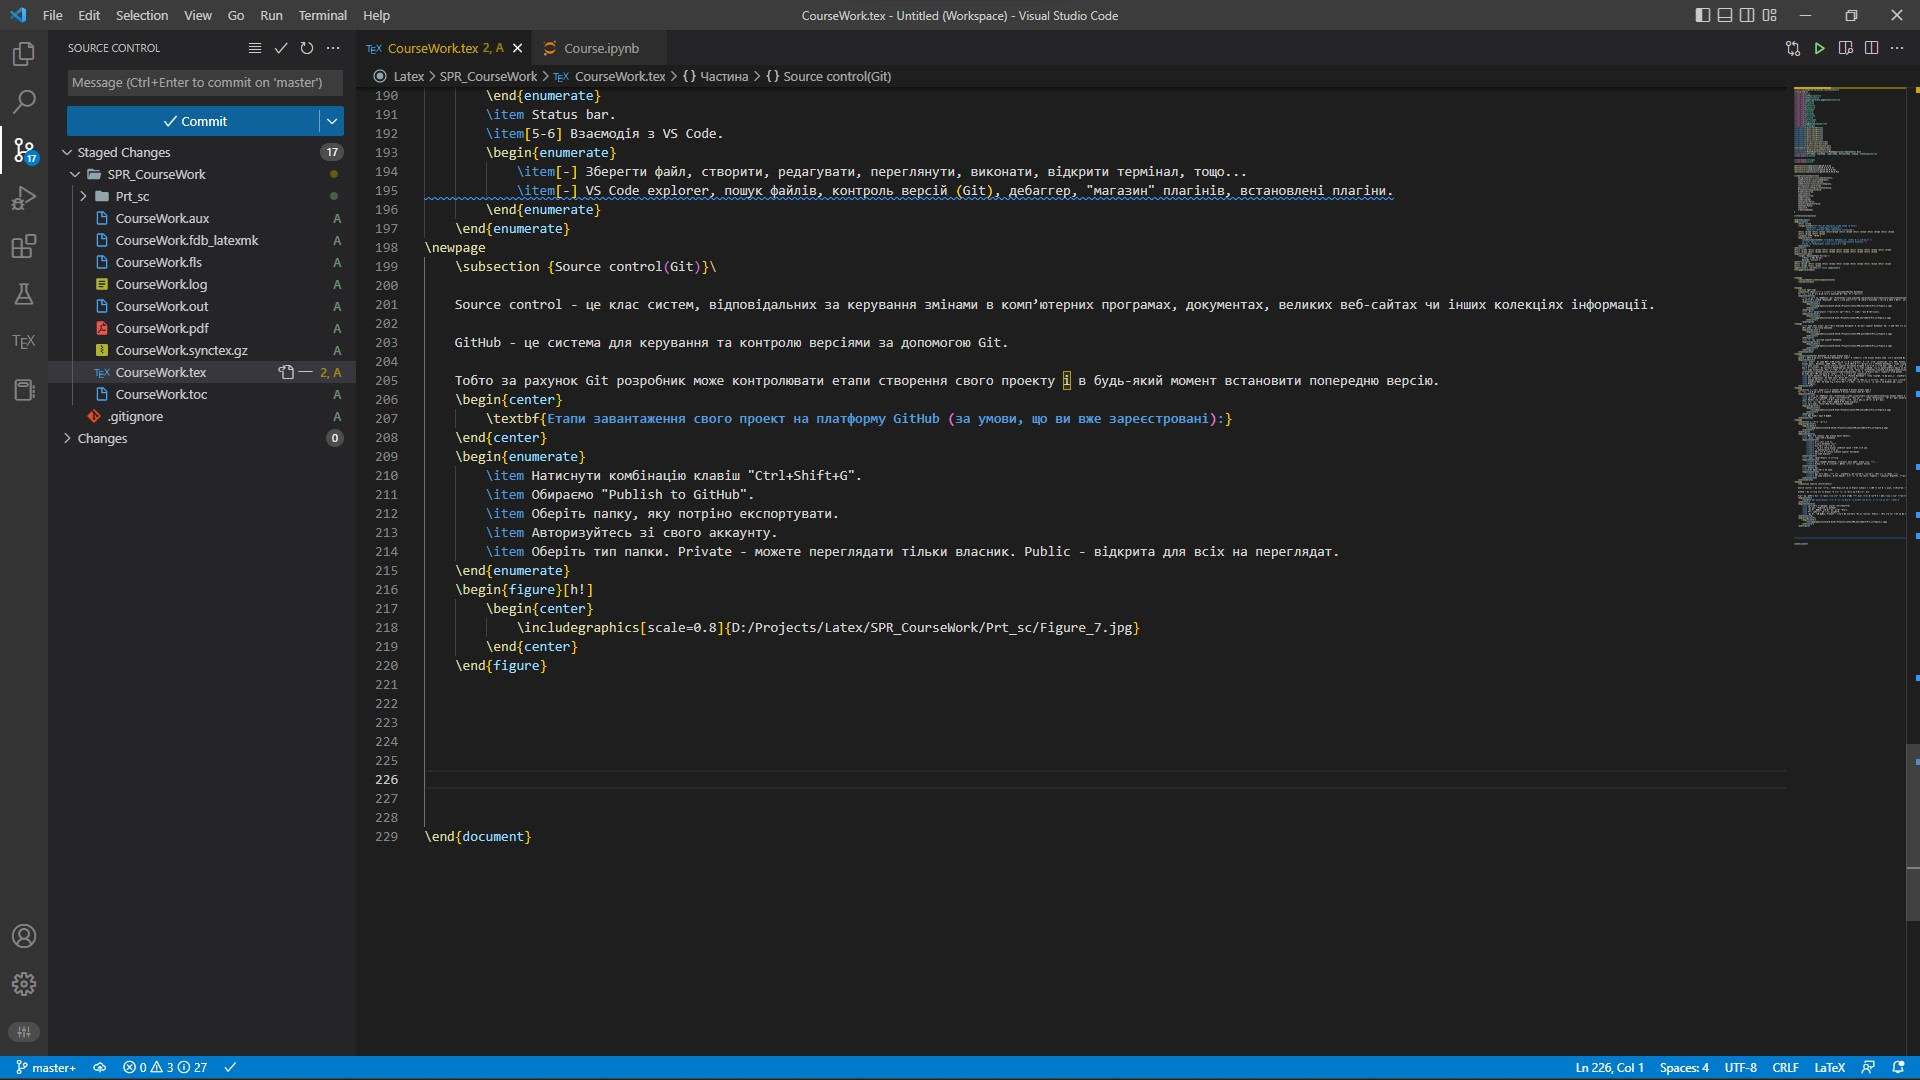
\includegraphics[width=1\linewidth]{Figure_8.jpg}  
		\end{minipage}
		\caption{Таблиця Subdivision05 перейменована на Subdivision.}
	\end{figure}
	
	
	
	
	
	
\newpage
		\begin{figure}[h!]
		\begin{center}
			\begin{minipage}[h]{1.05\linewidth}
				\includegraphics[width=1\linewidth]{Database Diagram.jpg}
			\end{minipage}
		\end{center}
		\caption{Entity relationship diagram}
	\end{figure}
	
	
	
\end{document}